\newpage
\section{Anhang}

\subsection{Anforderungsliste}\label{anforderungliste}
Die erste Version der Anforderungsliste ist nachfolgend angehängt.

\begin{table}[H]
\centering
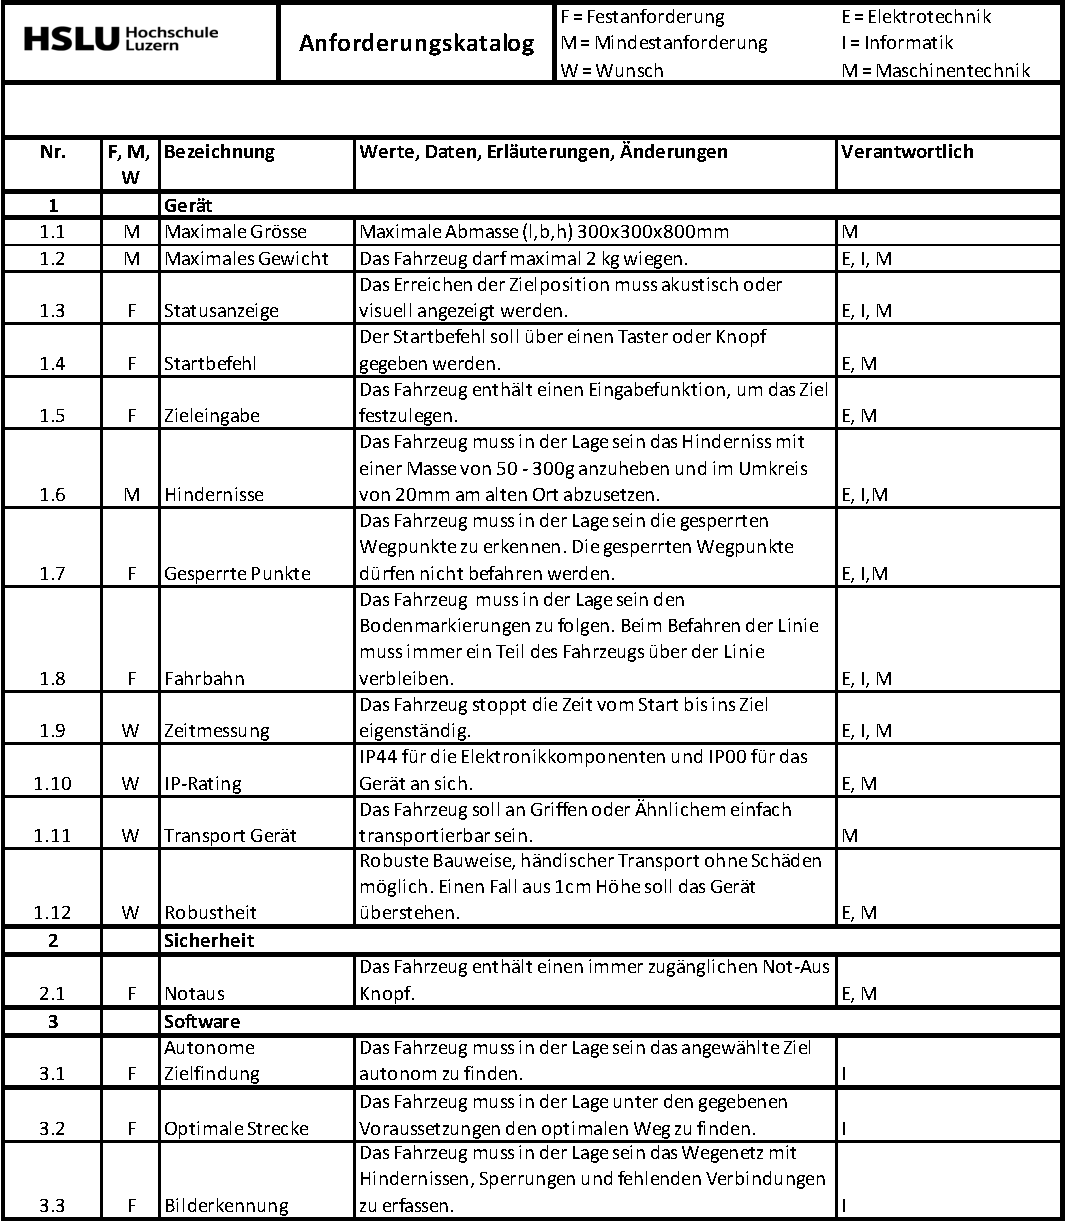
\includegraphics[width=\textwidth]{assets/Anforderungsliste_V1.01_page1.pdf}
\caption{Anforderungsliste Teil 1}
\label{table:anforderungsliste_page1}
\end{table}
\newpage

\begin{table}[H]
\centering
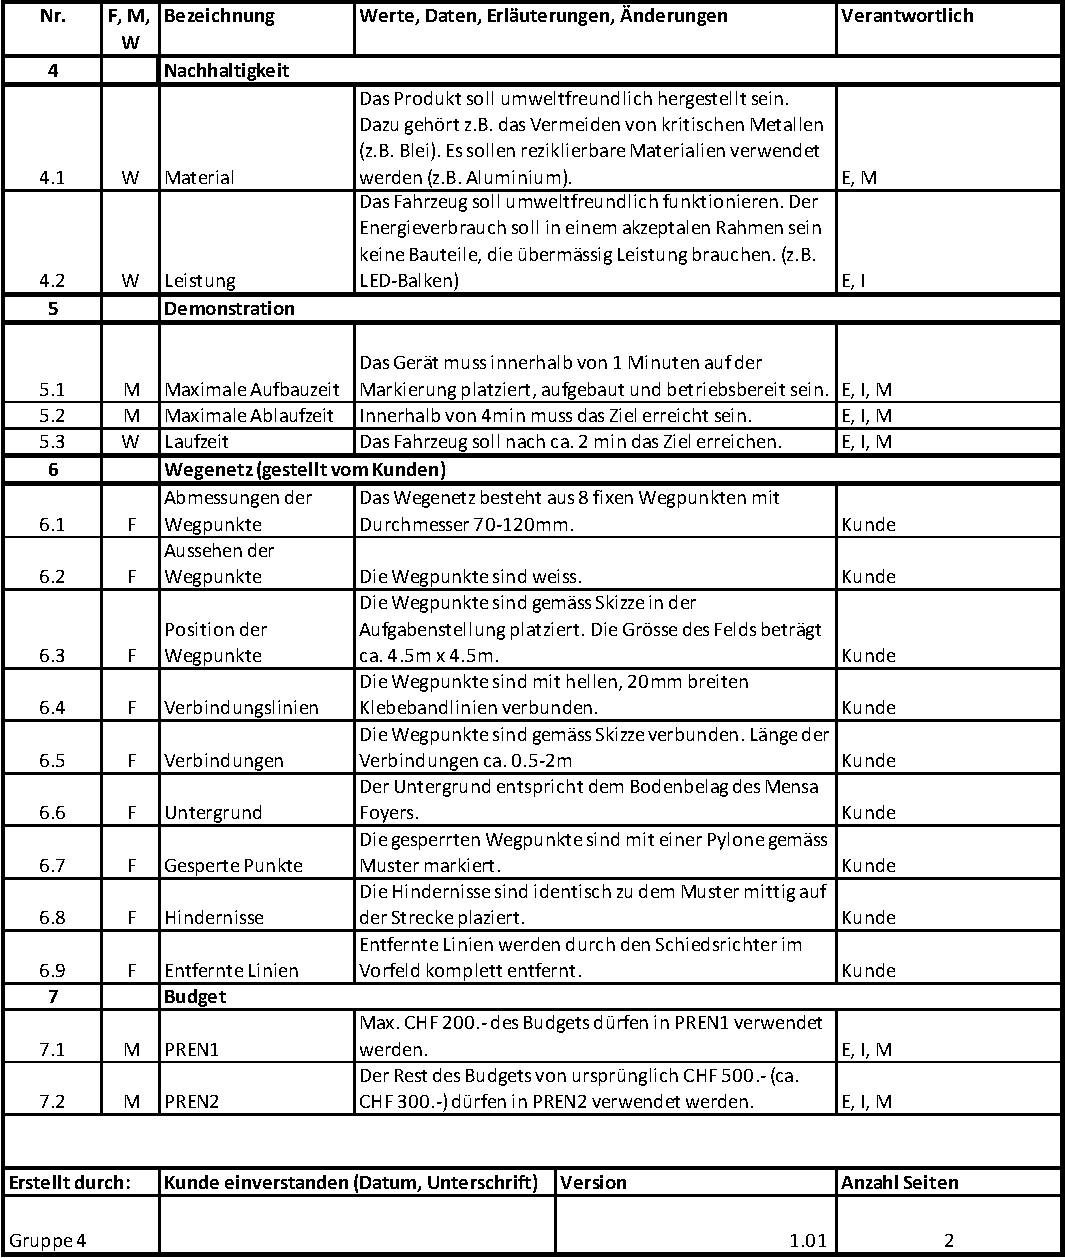
\includegraphics[width=\textwidth]{assets/Anforderungsliste_V1.01_page2.pdf}
\caption{Anforderungsliste Teil 2}
\label{table:anforderungsliste_page2}
\end{table}
\newpage

\begin{landscape}
\subsection{Kommunikationsplan}\label{kommunikationsplan}
Die Kommunikationskanäle sind folgendermassen definiert:

\begin{table}[H]
\centering
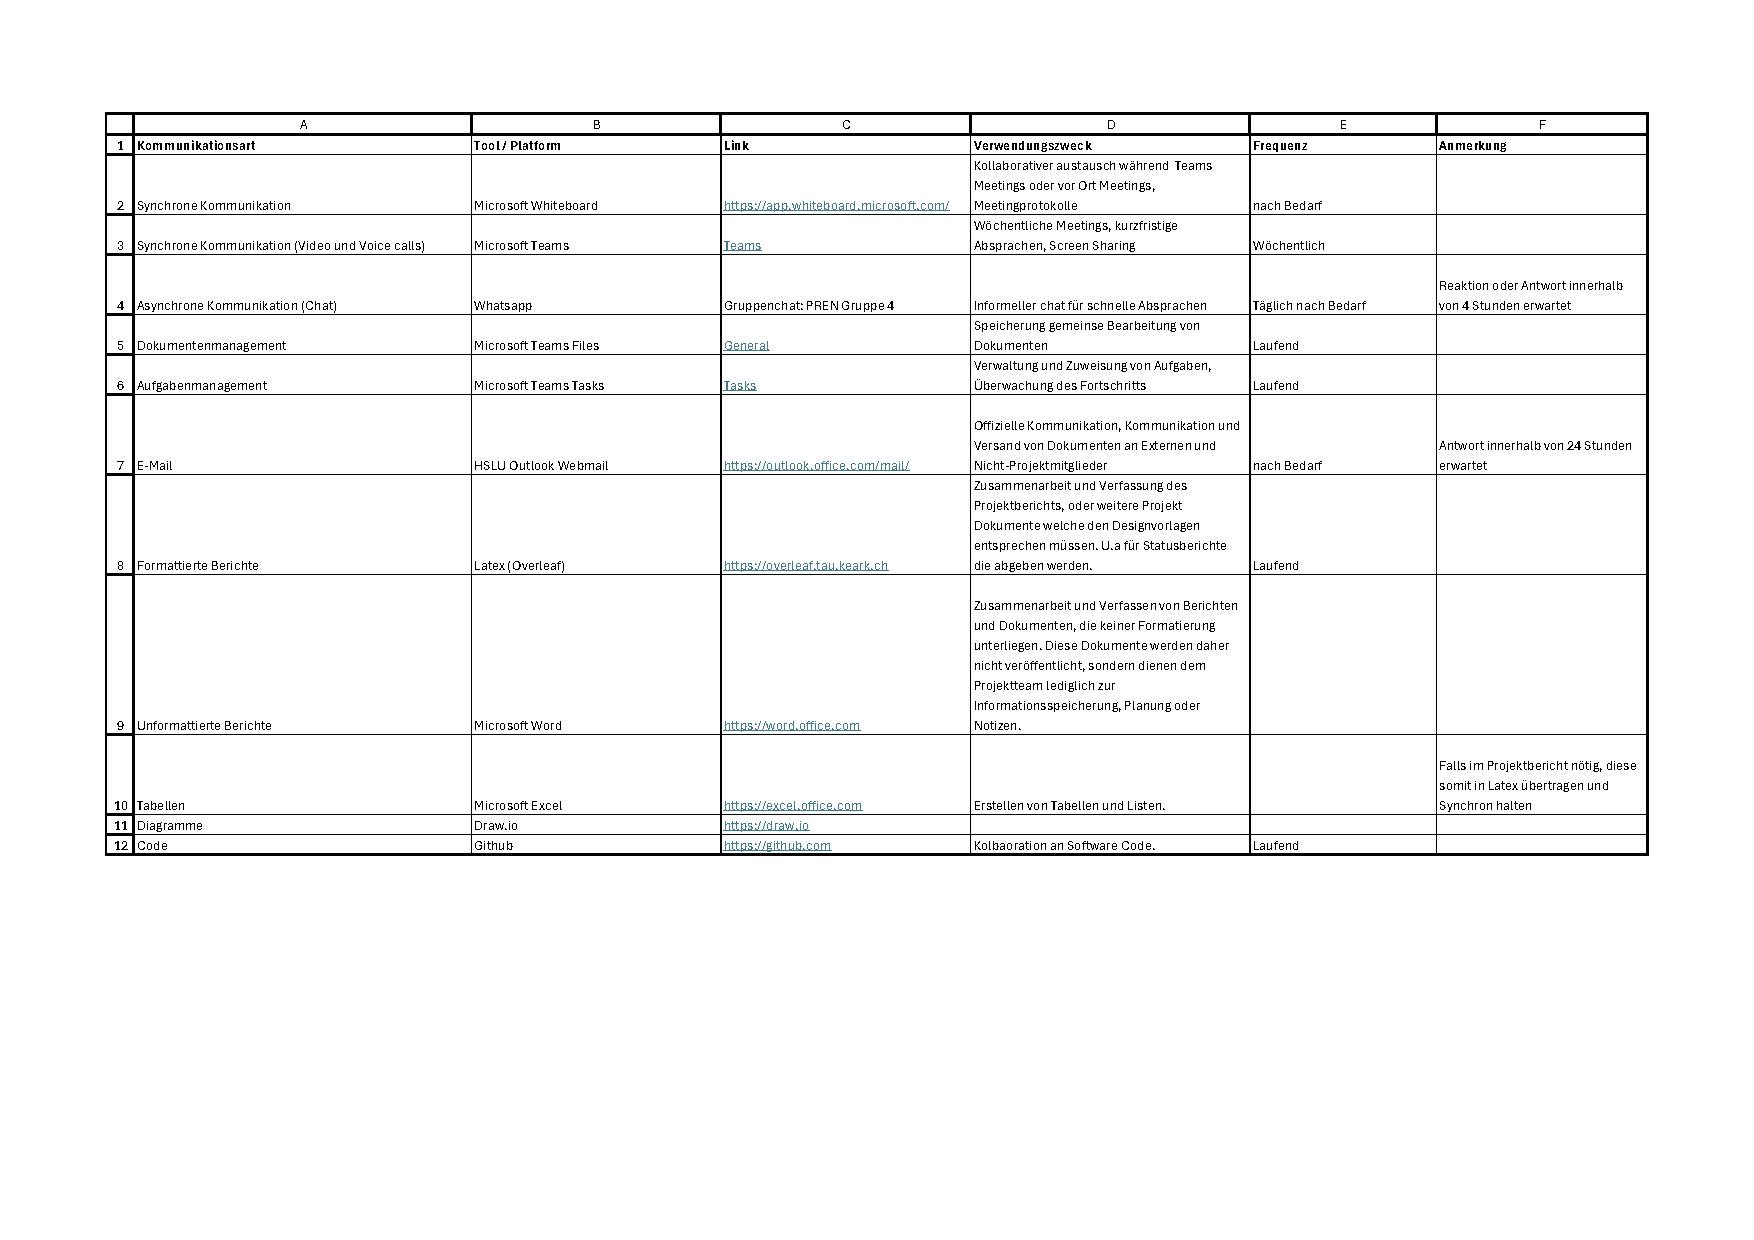
\includegraphics[width=240mm]{assets/Kommunikationschnittstellen.pdf}
\caption{Kommunikationsplan}
\label{table:communications-plan}
\end{table}
\end{landscape}

%%%%%%%%%%%%%%%%%% Technologierecherche %%%%%%%%%%%%%%%%%%%%

\subfile{parts/a-technologierecherchen}


%%%%%%%%%%%%%%%%%%%%%%%%%%%%%%%%%%%%%%%%%%%%%
%%%%%%% Entfernt, weil bereits in Doc   %%%%%
%%%%%%%%%%%%%%%%%%%%%%%%%%%%%%%%%%%%%%%%%%%%%
%\subsection{Morphologischer Kasten}\label{Morphologischer Kasten}
%Nachfolgend die Morphologischen Kästen, unterteilt in die jeweiligen Studiengänge, Elektrotechnik, Informatik und Maschinentechnik. %Jeder Kasten hat 3 Varianten eingezeichnet. Variante A: Gelb, Variante B: Rot, Variante C: Grün.
%
%\begin{table}[H]
%\centering
%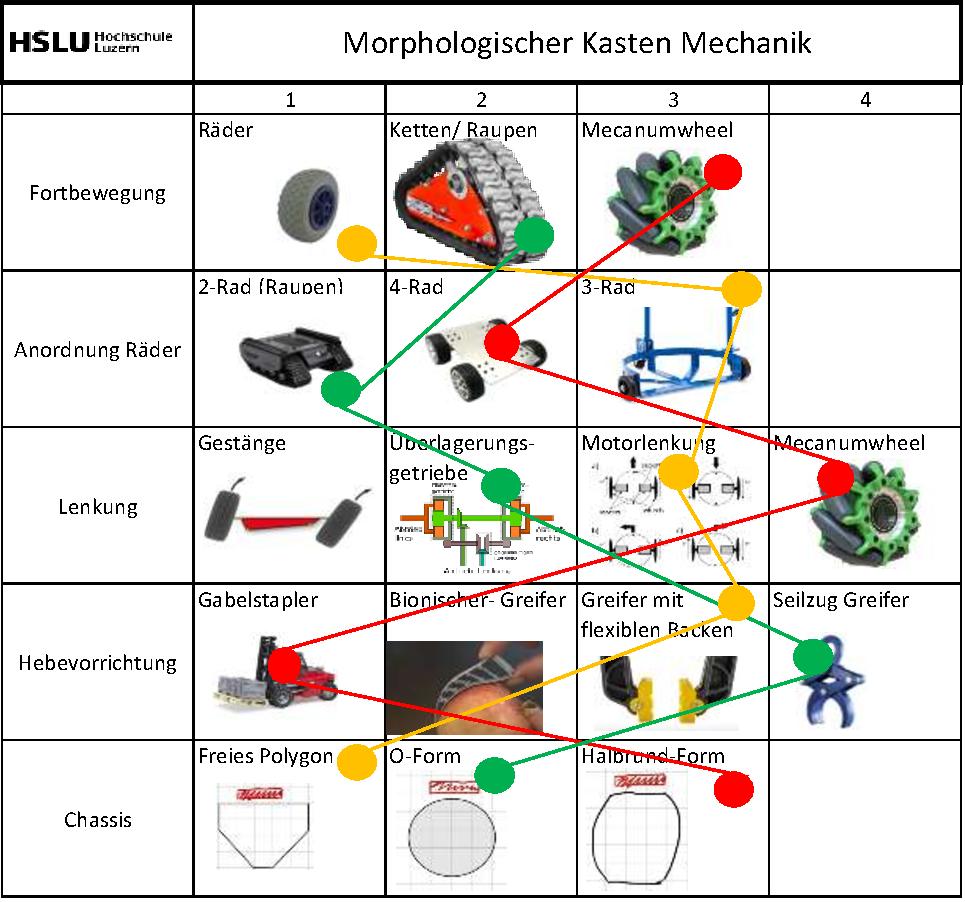
\includegraphics[width=\textwidth]{assets/MK_Maschinentechnik.pdf}
%\caption{Morphologischer Kasten: Maschinentechnik}
%\label{table:MK-Maschinentechnik}
%\end{table}
%\newpage
%\begin{table}[H]
%\centering
%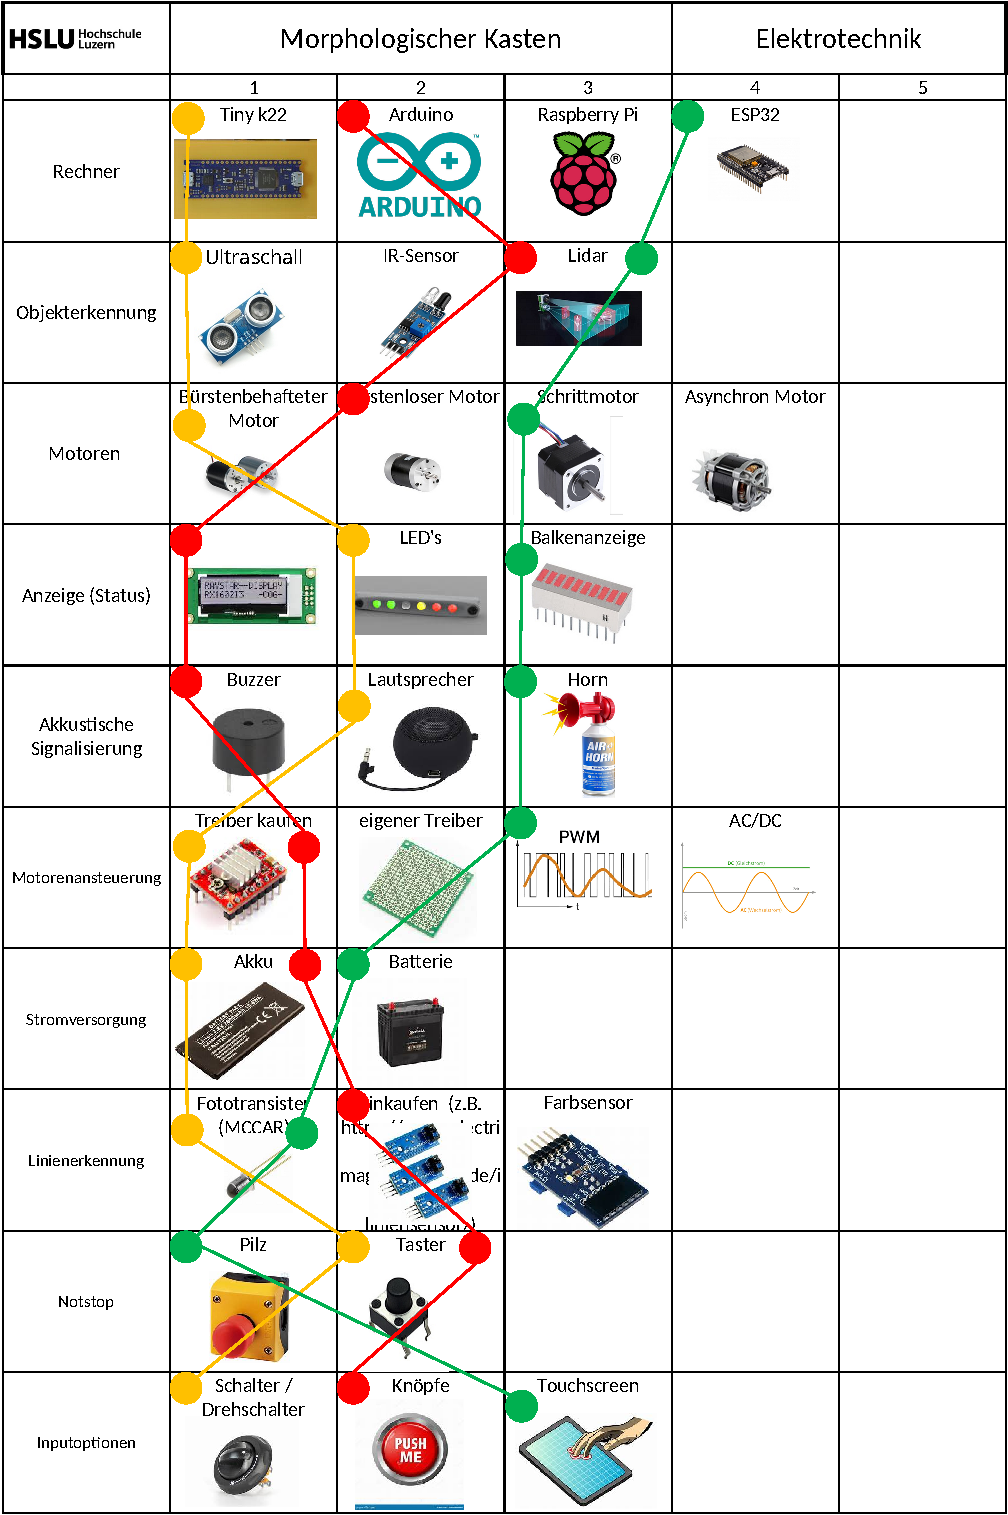
\includegraphics[height=\textheight-1cm]{assets/MK_Elektrotechnik.pdf}
%\caption{Morphologischer Kasten: Elektrotechnik}
%\label{table:MK-Elektrotechnik}
%\end{table}
%\newpage
%\begin{table}[H]
%\centering
%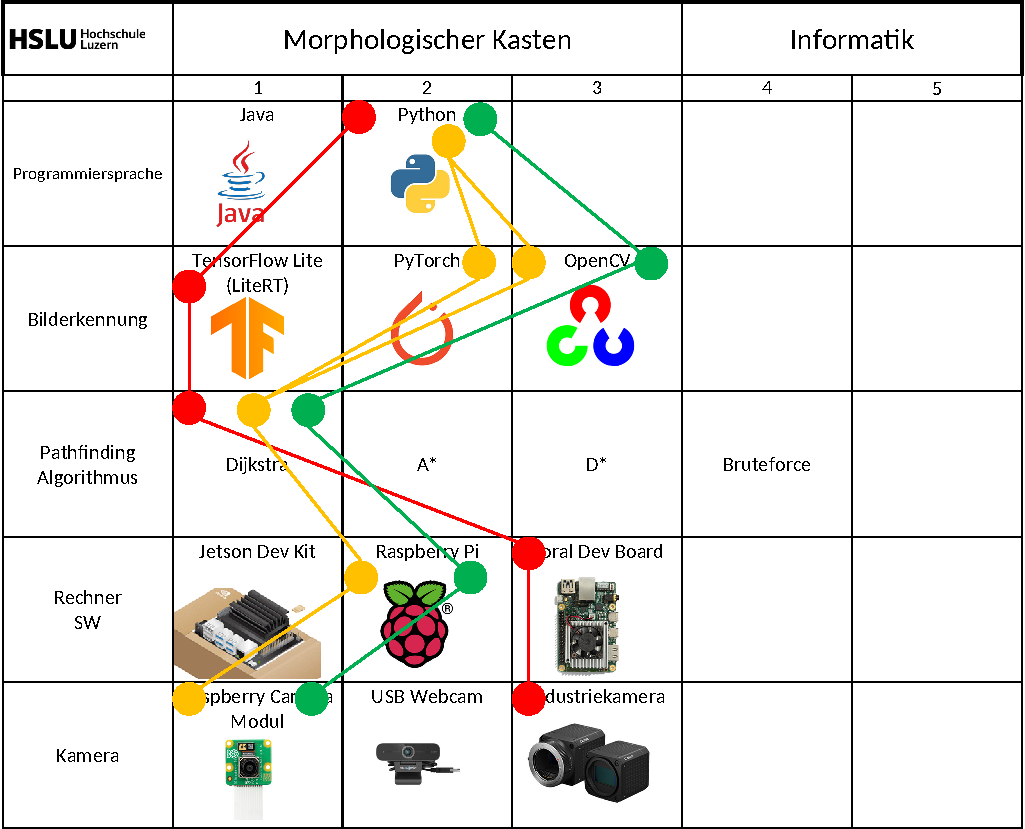
\includegraphics[width=\textwidth]{assets/MK_Informatik.pdf}
%\caption{Morphologischer Kasten: Informatik}
%\label{table:MK-Informatik}
%\end{table}
%\newpage
%\begin{table}[H]
%\centering
%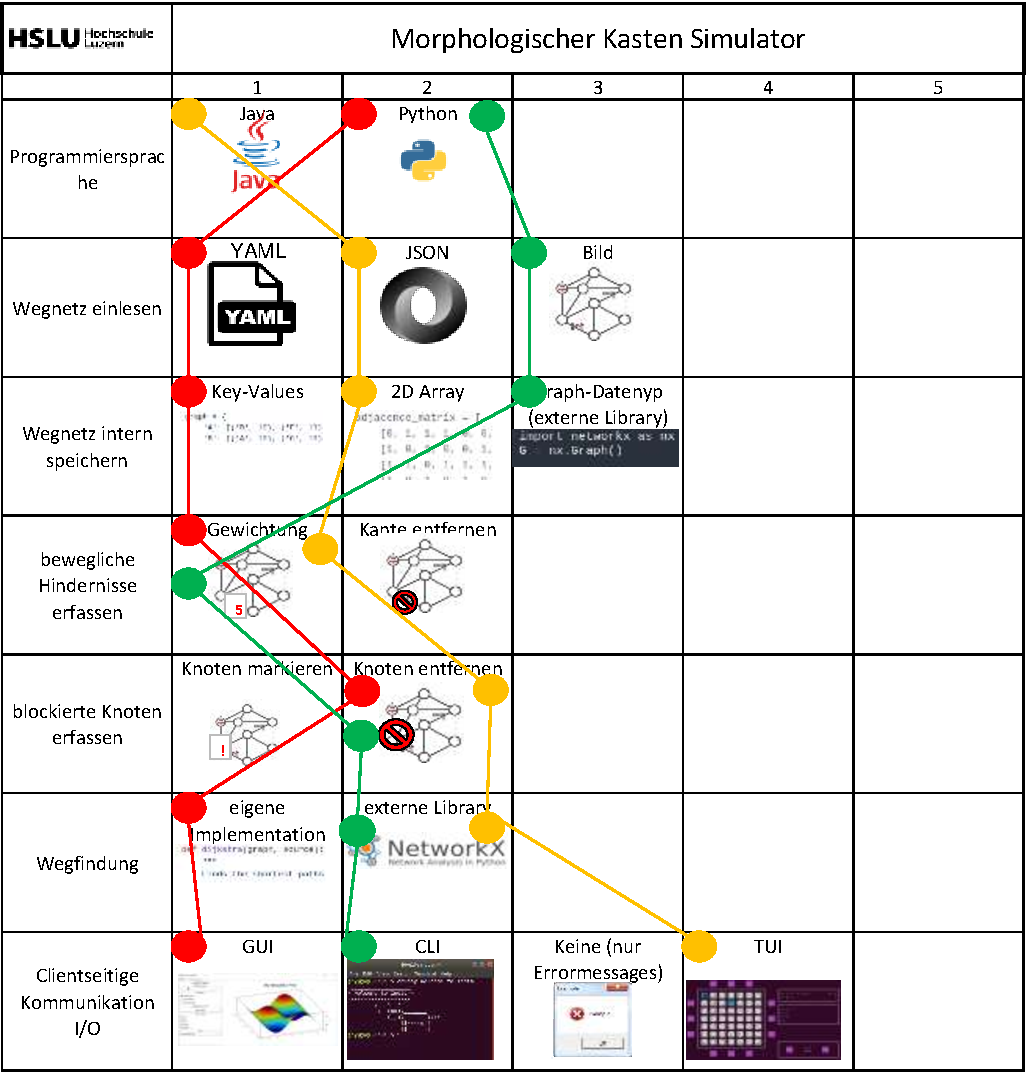
\includegraphics[width=\textwidth]{assets/MK_Simulator.pdf}
%\caption{Morphologischer Kasten: Simulator}
%\label{table:MK-Simulator}
%\end{table}
%\newpage


%%% THIS IS USELESS %%%%%%%%%%%%

% \subsection{Originale Aufgabenstellung}\label{aufgabenstellung}

% Nachfolgend ist die originale Aufgabenstellung angehängt.

% 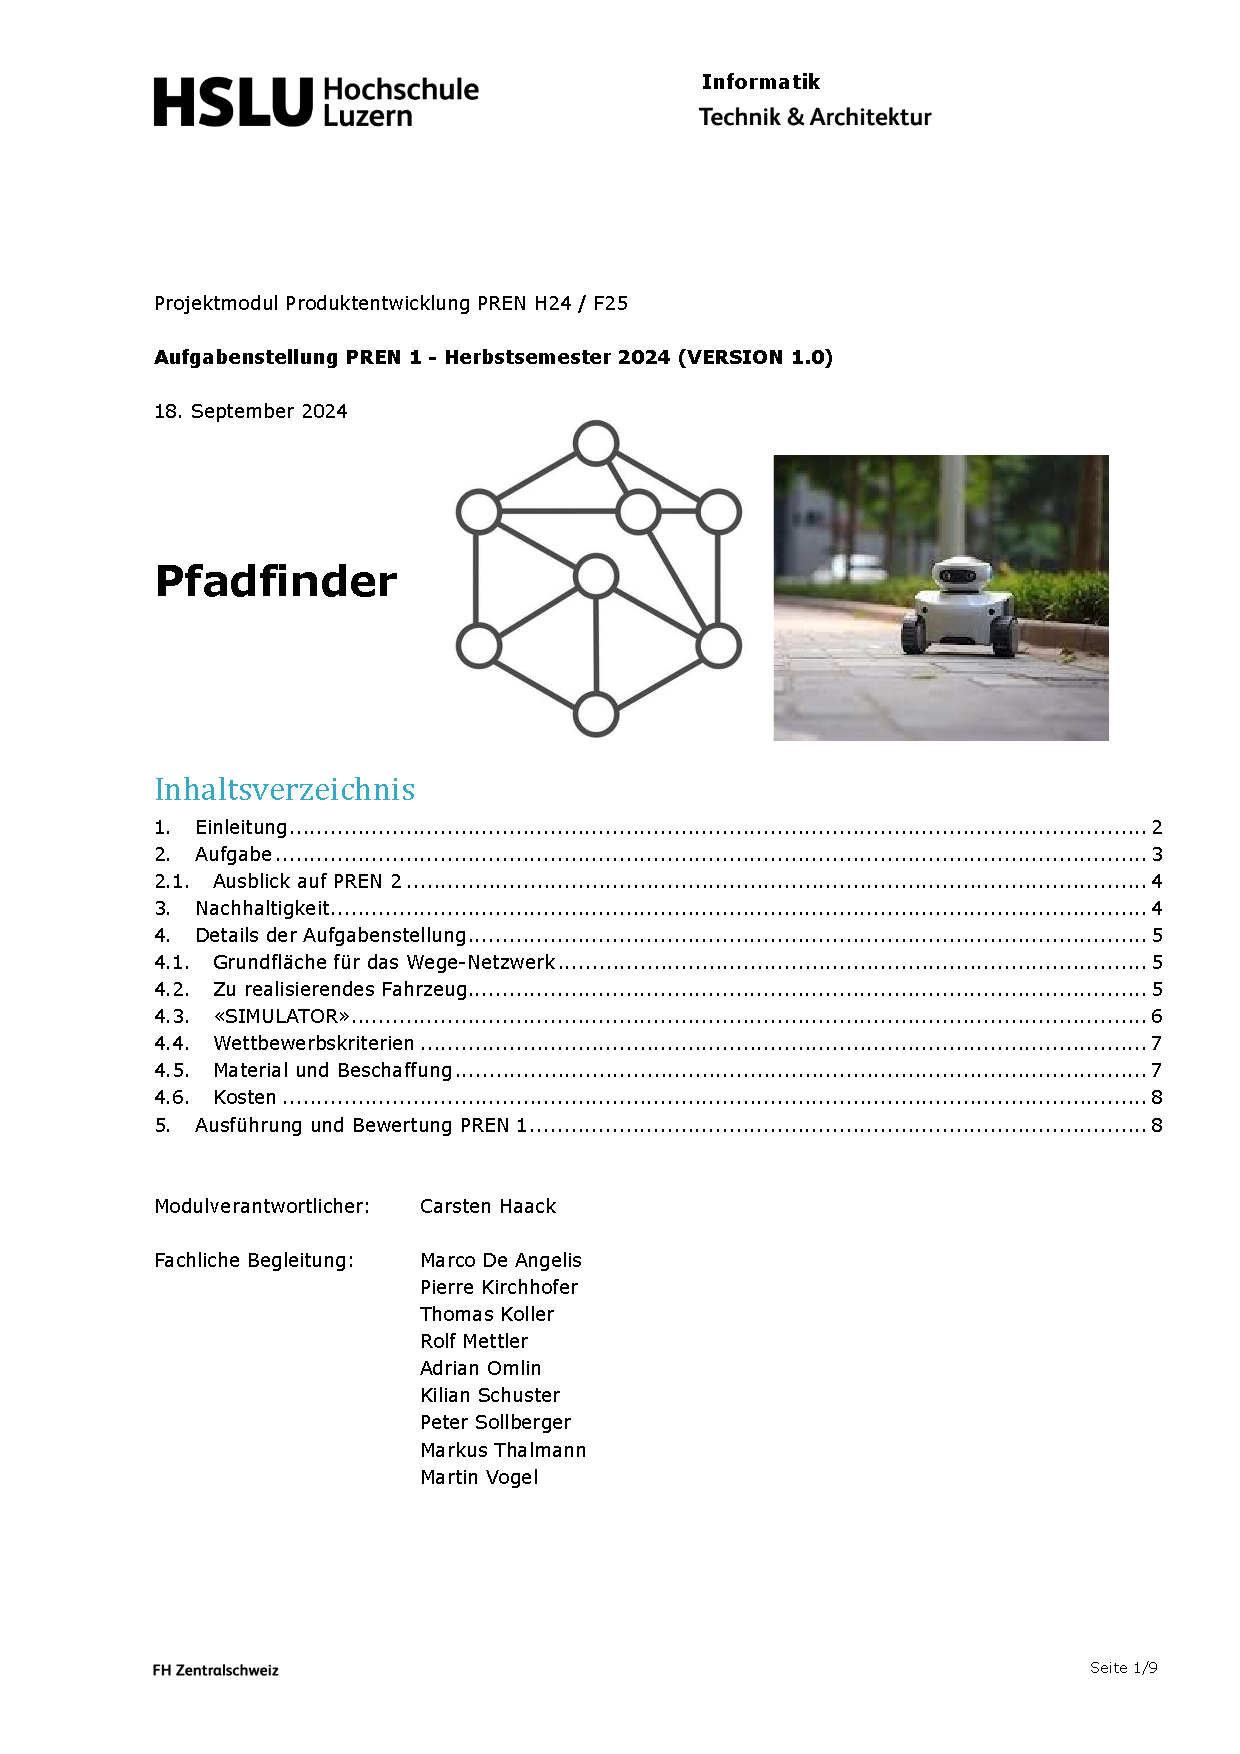
\includepdf[pages=-]{assets/AufgabenstellungPREN1HS24.pdf}
